%%%%%%%%%%%%%%%%%%%%%%%%%%%%%%%%%%%%%
%Presentazione esame di Dottorato Davide Spataro
%introduction.tex
%Purpose: This file contains the introduction to the problem the thesis tries to solve, it shows why single chip performances are not improving as much as the moore's law predicts and introduces the concept of parallelism in computation and in numerical simulation.
%@author Davide Spataro
%@version 1.0 14/01/2018 Eindhoven
%%%%%%%%%%%%%%%%%%%%%%%%%%%%%%%%%%%%

\section[Conclusion]{Conclusion}
%%%%%%%%%%%%%%%%%%%%%%%%%%%%%%%%%%%%
\frame{\frametitle{Conclusion}
	\begin{block}{Main thrust of this work}
		\begin{itemize}
			\item design of a programming abstraction for 
			\item CA and FDM targeting many-core heterogeneous HW
			\item from commodity PC to large computing cluster of accelerators
		\end{itemize}
		\end{block}	
				\begin{block}{\textbf{Write once} $\longrightarrow$ \textbf{Execute everywhere}}
			\item Domain Specific Language + Dedicated Libraries 
			\begin{itemize}
				\item shared-memory (OpenMP)
				\item \textit{GPUs/Intel Phi/FPGA} $\ldots$
				\item \textbf{Distributed Memory + multi-accelerators}
				\item Programming effort is considerably reduced 
			\end{itemize}
		\end{block}	
	}
\frame{\frametitle{Conclusion - Other Applications of OpenCAL}
			OpenCAL was adopted (among other works), in the context of this work for:
			\begin{itemize}
				\item  the \textbf{tracking of bacteria} from the analysis of time-lapse video 
				\item the modeling of \textbf{Bird Flock Dynamics}
				\pause
				\item Both works that have been originally developed within the context of OpenCAL  but have developed over time into something self-contained.
			\end{itemize}
			\begin{figure}
				\centering
				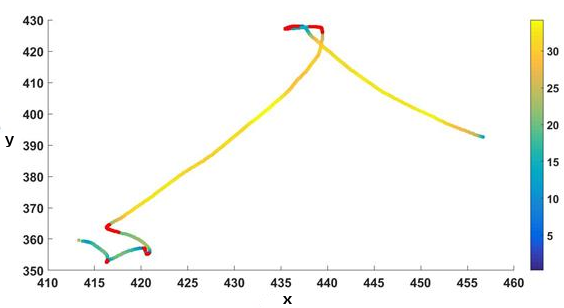
\includegraphics[width=0.6\textwidth]{images/runtumble}
				\caption{Example of a tracked bacterium trajectory}
			\end{figure}
		
	
}

%

